\chapter{力、位相空間、保存則}

\lectureoverview{運動法則は、なじみ深い物理量を関係づけるだけでは不十分である。系の状態を指定し、その状態をある瞬間から次の瞬間へ運び、運動を経てもなお生き残る区別と量を示さなければならない。まずもっともらしいが誤った力の法則を検証し、次に状態を位置から位相空間へ拡大し、最後に運動量とエネルギーの保存を導くことによって、ニュートン力学に到達する。}

\section{有用な誤った法則}

日常の運動は摩擦に支配されている。重い物体を床の上で押せば動き、押すのをやめればまもなく止まる。より大きな力で押せば一般により大きな速さが生じ、より重い物体にはより強い押しが必要である。そのような世界では、力が速度そのものを生み出すと考えるのは自然である。これがアリストテレス的な運動記述の背後にあった基本的な直観であった。

アイススケートは欠けていた経験を与えてくれる。スケーターは動き始める、止まる、方向を変えるためには力を必要とするが、いったん動き出した後は滑り続けるために力を必要としない。もしアリストテレスが普通の地面ではなくほとんど摩擦のない氷の上で仕事をしていたなら、力--速度という直観の欠陥ははるかに見逃しにくかったであろう。

その直観のどこが誤っているかを明らかにするために、それに精密な現代的形態を与えよう。故意に誤った方程式を書く。

\begin{equation}
  \mathbf F=m\mathbf v.
  \label{eq:aristotle-vector-law}
\end{equation}

これはニュートンの法則ではなく、物理学として暗記されるべきものではない。その価値は診断的である。言葉による規則が方程式になれば、それが運動を予測するかどうか、また過去を再構成するのに十分な情報を保存するかどうかを問うことができる。力に当たるギリシア語についての短い教室での議論は\emph{デュナミス}を指し示す。これはダイナモやダイナミクスといった語にも聞かれる語根であるが、用語法は法則そのものの検証にとって二次的なものである。

\begin{figure}[htbp]
  \centering
  \includegraphics[width=0.82\textwidth]{lecture_02_figure_02.png}
  \caption{予測可能性と可逆性を検証するために用いられる、意図的に誤った力--速度の法則。}
  \lectureframe{00:04:51}
\end{figure}

運動を一次元の空間座標に制限する。\(v=\dot x\)であるから、法則は

\begin{equation}
  F(t)=m\dot x(t).
  \label{eq:aristotle-1d}
\end{equation}

次に時間を長さ\(\delta\)の短い区間に分割する。一区間にわたって、

\begin{equation}
  \dot x(t)\simeq
  \frac{x(t+\delta)-x(t)}{\delta}.
  \label{eq:first-difference}
\end{equation}

式~\eqref{eq:aristotle-1d}に代入すると

\begin{equation}
  x(t+\delta)
  =x(t)+\frac{\delta}{m}F(t).
  \label{eq:aristotle-update}
\end{equation}

これは本物の更新規則の形をしている。現在の位置と力がわかれば、次のストロボスコープ的な瞬間の位置が従う。しかし力が消えると、アリストテレスの規則は\(\dot x=0\)を与える。すなわち物体は静止したままでなければならない。支える力のない運動は初めから排除されている。

\begin{figure}[htbp]
  \centering
  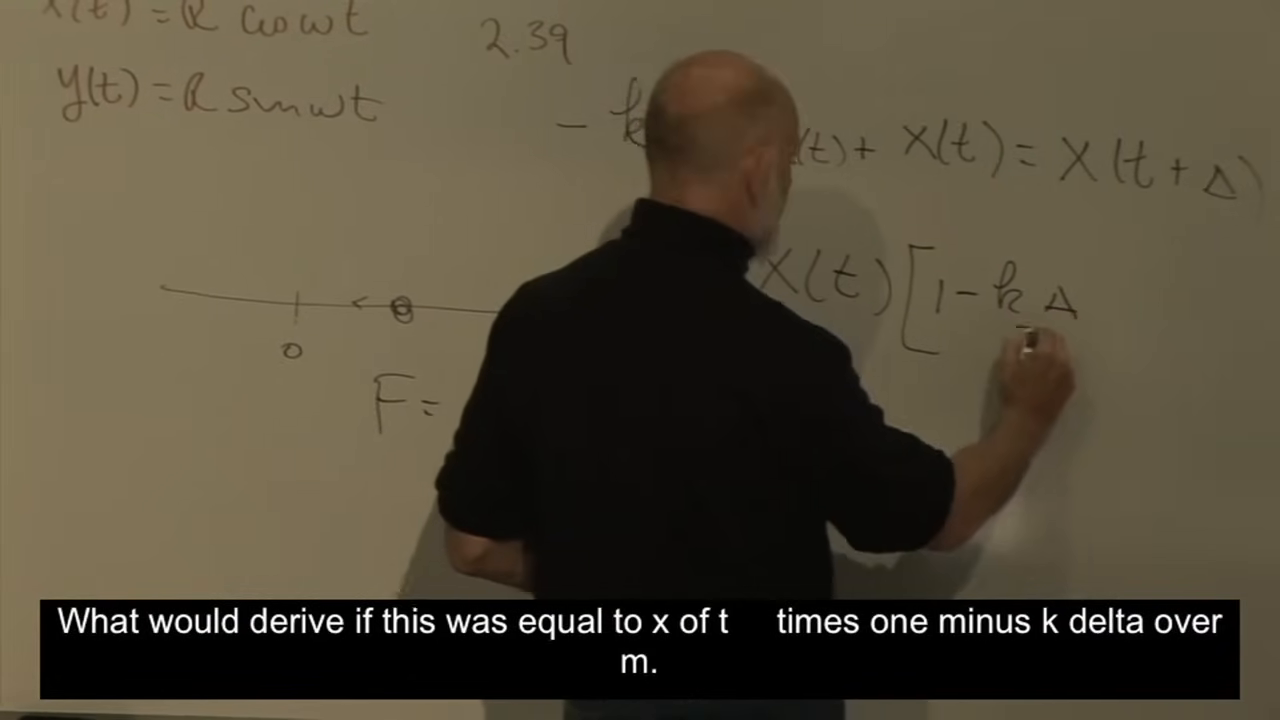
\includegraphics[width=0.84\textwidth]{lecture_02_figure_07.png}
  \caption{復元力を伴う離散的なアリストテレスの更新。各ステップは変位を1よりわずかに小さい因子で掛ける。}
  \lectureframe{00:10:15}
\end{figure}

\subsection{アリストテレス力学におけるばね}

ばねに取り付けられた粒子を考え、つり合いの位置を\(x=0\)とする。変位は復元力を生み、

\begin{equation}
  F(x)=-kx,
  \qquad k>0.
  \label{eq:hooke-law}
\end{equation}

この力を式~\eqref{eq:aristotle-update}に代入すると次を得る。

\begin{equation}
  x(t+\delta)
  =\left(1-\frac{k\delta}{m}\right)x(t).
  \label{eq:aristotle-spring-update}
\end{equation}

十分に小さい\(\delta\)に対して、括弧内の因子は1のすぐ下にある。したがって各更新は変位を同じ割合だけ減少させる。

\begin{equation}
  x_n=\left(1-\frac{k\delta}{m}\right)^n x_0.
  \label{eq:aristotle-geometric-decay}
\end{equation}

連続的な方程式とその解は

\begin{align}
  m\dot x&=-kx,
  \label{eq:aristotle-spring-continuous}\\
  x(t)&=x(0)e^{-kt/m}.
  \label{eq:aristotle-spring-solution}
\end{align}

ばねは振動しない。どのような変位から放たれても、原点に指数的に近づき、近づくにつれてますますゆっくりと動く。

\begin{figure}[htbp]
  \centering
  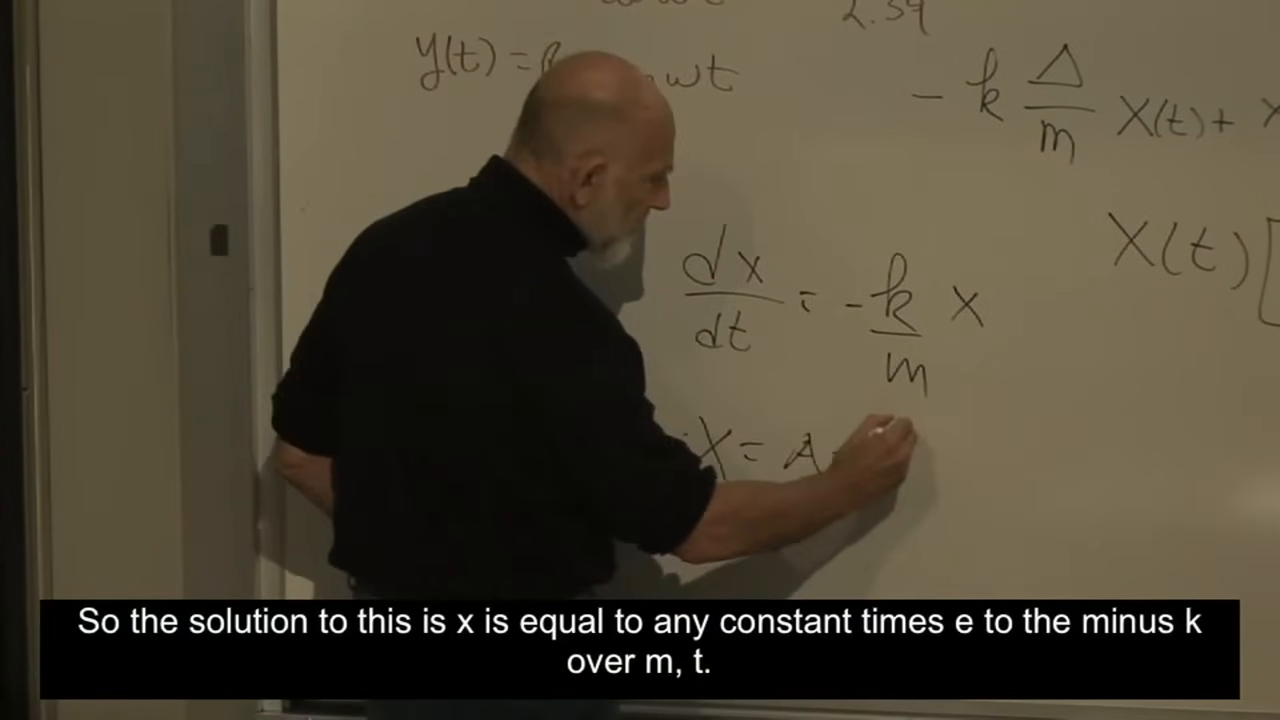
\includegraphics[width=0.84\textwidth]{lecture_02_figure_08.png}
  \caption{アリストテレスのばね方程式の指数解。変位は振動せずに減衰する。}
  \lectureframe{00:12:02}
\end{figure}

未来を予測するのは容易である。どの初期変位も同じ静止配置に近づく。過去は別問題である。粒子が原点のごく近くで有限の精度でしか観測されないとしよう。それは多くの異なる変位のいずれから始まっていてもよい。それらの指数的に小さな名残はすべて、やがて同じ測定許容範囲内に収まるからである。完全な数学的精度があれば式~\eqref{eq:aristotle-spring-solution}は逆向きに走らせることができるが、履歴間の実際的な区別は着実に消去される。したがってこの法則は、可逆な基礎力学の観点からは疑わしい。

これはアリストテレスが非理性的であったという意味ではない。彼が記述した摩擦に支配された運動は、実際に散逸的である。誤りは、その有効な振る舞いを基礎法則に格上げしたことにあった。摩擦それ自体、複雑な微視的相互作用から生じる一つの力である。手が物体をほぼ一定の速さで押すとき、加えられた力は摩擦とつり合っているのであり、加えられた力が速度そのものを生み出しているのではない。

\section{ニュートンの法則とその物理的意味}

ニュートンによる修正は、力が運動を変化させるというものである。

\begin{equation}
  \mathbf F=m\mathbf a=m\ddot{\mathbf x}.
  \label{eq:newton-second-law}
\end{equation}

これを発展方程式として扱う前に、二つの見かけ上の循環を解きほぐさなければならない。第一は基準系に関するものである。ニュートンの法則は慣性系で成り立ち、慣性系とはニュートンの法則が成り立つ系である、とよく言われる。物理的な主張はその循環的な定義ではない。適切な棒と時計で記述される、ニュートンの法則がその単純な形をとるような系が\emph{存在する}という経験的な主張である。それらに対して加速または回転する系では、追加の見かけの力が必要となる。それらの他の系で方程式がどのように変換されるかは、後で計算できる。

第二の循環は力と質量に関するものである。力が質量掛ける加速度と定義され、質量が力割る加速度と定義されるなら、その方程式は空虚に見える。操作的な実験が定義を法則から分離する。物体を標準キログラムと釣り合わせて比較し、次にその物体を、他に力のない空間でばね秤に取り付ける。力の一単位を、ばねの固定された小さな伸びによって定義する。同じ量だけ伸びた二本の同一のばねは、二単位の力を与え、二倍の加速度を生じる。一本のばねを二倍の距離だけ伸ばすよりも、二本目のばねを追加する方が安全である。なぜなら、実際のばねはやがて非線形になるか、壊れるからである。一本のばねを保ちながら二つの等しい質量を結合すると、加速度は半分になる。三つの等しい質量では三分の一になる。

\begin{figure}[htbp]
  \centering
  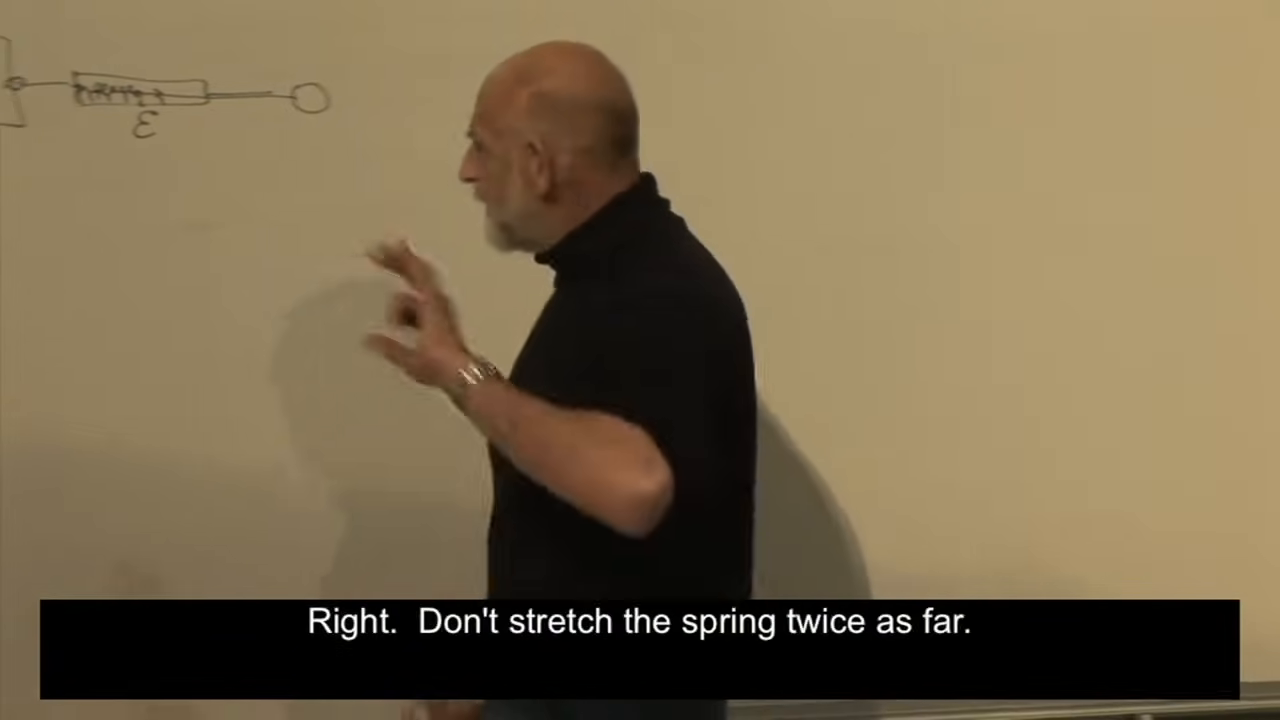
\includegraphics[width=0.84\textwidth]{lecture_02_figure_09.png}
  \caption{力の等しい単位を定義し、加速度が力に比例することを検証するために用いられたばね秤の思考実験。}
  \lectureframe{00:22:45}
\end{figure}

これらの比較は、経験的な内容を次に与える：

\begin{equation}
  a\propto F,
  \qquad
  a\propto\frac{1}{m},
  \qquad
  F=ma.
  \label{eq:force-mass-scaling}
\end{equation}

\emph{粒子}という語は、内部構造が無関係であるような任意の小さな物体に対して用いられ、素粒子だけに対して用いられるのではない。

\subsection{なぜ位置だけでは状態にならないか}

ここで、同じストロボスコープ法によってニュートンの方程式を検証する。加速度に対する中心差分は

\begin{equation}
  \ddot x(t)\simeq
  \frac{x(t+\delta)-2x(t)+x(t-\delta)}{\delta^2}.
  \label{eq:second-difference}
\end{equation}

したがって、ニュートンの方程式は次を意味する：

\begin{equation}
  x(t+\delta)
  =2x(t)-x(t-\delta)+\frac{\delta^2}{m}F(t).
  \label{eq:newton-position-update}
\end{equation}

次の位置は\(x(t)\)だけからは得られない。前の位置\(x(t-\delta)\)、あるいは同等に現在の瞬間における速度も必要である。一見すると、これはニュートンの方程式をアリストテレスのものよりも予測力が低いものに見せる。しかし正しい結論は、位置だけでは状態の不完全な記述であったということである。ある瞬間に関連するすべてを知るとは、その後の運動を決定するのに十分なデータを知ることを意味する。ニュートン的な粒子に対して、それらのデータは位置と速度である。

\section{運動量と位相空間}

運動量を次によって導入する：

\begin{equation}
  \mathbf p=m\mathbf v=m\dot{\mathbf x}.
  \label{eq:momentum-definition}
\end{equation}

固定されたニュートン系の質量は一定とみなされる。物体は、ペンがそのキャップを失うように、一部を失うことがあるが、その場合記述されている物体は変化しており、選ばれた閉じた系は依然として一定の全質量を持つ。一定の\(m\)のもとで、ニュートンの第二法則は次になる：

\begin{equation}
  \mathbf F=\dot{\mathbf p}.
  \label{eq:newton-momentum-form}
\end{equation}

\begin{figure}[htbp]
  \centering
  \includegraphics[width=0.82\textwidth]{lecture_02_figure_03.png}
  \caption{運動量の時間微分として書かれたニュートンの法則。}
  \lectureframe{00:32:35}
\end{figure}

一つの座標に対して、ニュートン的運動は今や二つの独立な状態変数に対する二つの一階方程式として書ける：

\begin{align}
  \dot p&=F(x,t),
  \label{eq:first-order-p}\\
  \dot x&=\frac{p}{m}.
  \label{eq:first-order-x}
\end{align}

一方の方程式は力が運動量をどのように変えるかを述べ、他方は運動量が位置をどのように変えるかを述べる。それらの一階の離散形は

\begin{align}
  p(t+\delta)&=p(t)+\delta F(x(t),t)+O(\delta^2),
  \label{eq:momentum-discrete}\\
  x(t+\delta)&=x(t)+\frac{\delta}{m}p(t)+O(\delta^2).
  \label{eq:position-discrete}
\end{align}

\(x(t)\)と\(p(t)\)が与えられれば、これらの方程式は次の対を決定し、それが次に次のステップの入力となる。軌道は繰り返しの更新によって構築される。

\begin{figure}[htbp]
  \centering
  \includegraphics[width=0.84\textwidth]{lecture_02_figure_04.png}
  \caption{二つの一階方程式と対応する初期データ。位置と運動量がともに状態を指定する。}
  \lectureframe{00:35:47}
\end{figure}

すべての対\((x,p)\)の空間は\emph{位相空間}と呼ばれる。三次元を運動する一つの粒子に対して、それは六つの座標を持つ：

\begin{equation}
  (x,y,z,p_x,p_y,p_z).
  \label{eq:one-particle-phase-space}
\end{equation}

位相空間は完全な初期条件の空間である。配置空間は位置のみを記録し、位相空間は運動法則が必要とするデータを正確に記録する。

\begin{classroomqa}
  \audiencequestion{力が時間の既知の関数ではなく位置の関数である場合、更新はより複雑になるか？\lecturetimestamp{00:36:27--00:37:07}}
  \lecturerresponse{方程式は依然として予測的である。\(x\)と\(p\)が既知になれば、値\(F(x)\)が既知となる。式~\eqref{eq:first-order-p}は\(p\)を進め、式~\eqref{eq:first-order-x}は\(x\)を進め、更新された対を再び用いることができる。}
\end{classroomqa}

\section{ニュートンのばね}

二つの法則を同一の物理的基盤で比較できるように、ばねに戻る。ニュートンは次を与える：

\begin{equation}
  m\ddot x=-kx.
  \label{eq:newton-spring}
\end{equation}

定数を除くために一時的に\(m=k=1\)と置く。すると

\begin{equation}
  \ddot x=-x.
  \label{eq:normalized-oscillator}
\end{equation}

指数関数とは異なり、正弦または余弦は二回の微分の後で自身の負に戻る。一般解は次のように書ける：

\begin{align}
  x(t)&=C\cos(t-t_0),
  \label{eq:oscillator-x}\\
  p(t)=\dot x(t)&=-C\sin(t-t_0).
  \label{eq:oscillator-p}
\end{align}

この2つの定数は、初期情報の2つの部分を担っている。振幅\(C\)は最大変位を与え、一方\(t_0\)は位相を定める。ここでは\(t=t_0\)で速度が消えるように選んでいる。粒子は端点で一時的に停止するだけである。その後、原点を通って戻り、そこでは速さと運動量が最大になり、振動を続ける。

~\eqref{eq:oscillator-x} 式と \eqref{eq:oscillator-p} 式を二乗すると

\begin{equation}
  x^2+p^2=C^2.
  \label{eq:oscillator-phase-circle}
\end{equation}

したがって、位相空間の点は半径\(C\)の円上を動く。異なる初期振幅は異なる円を生み出す。\(t_0\)を変えると、同じ円上の異なる出発点が選ばれる。どの円も、この規格化された単位では振幅に依存せず、同じ周期\(2\pi\)で一周される。

\begin{figure}[htbp]
  \centering
  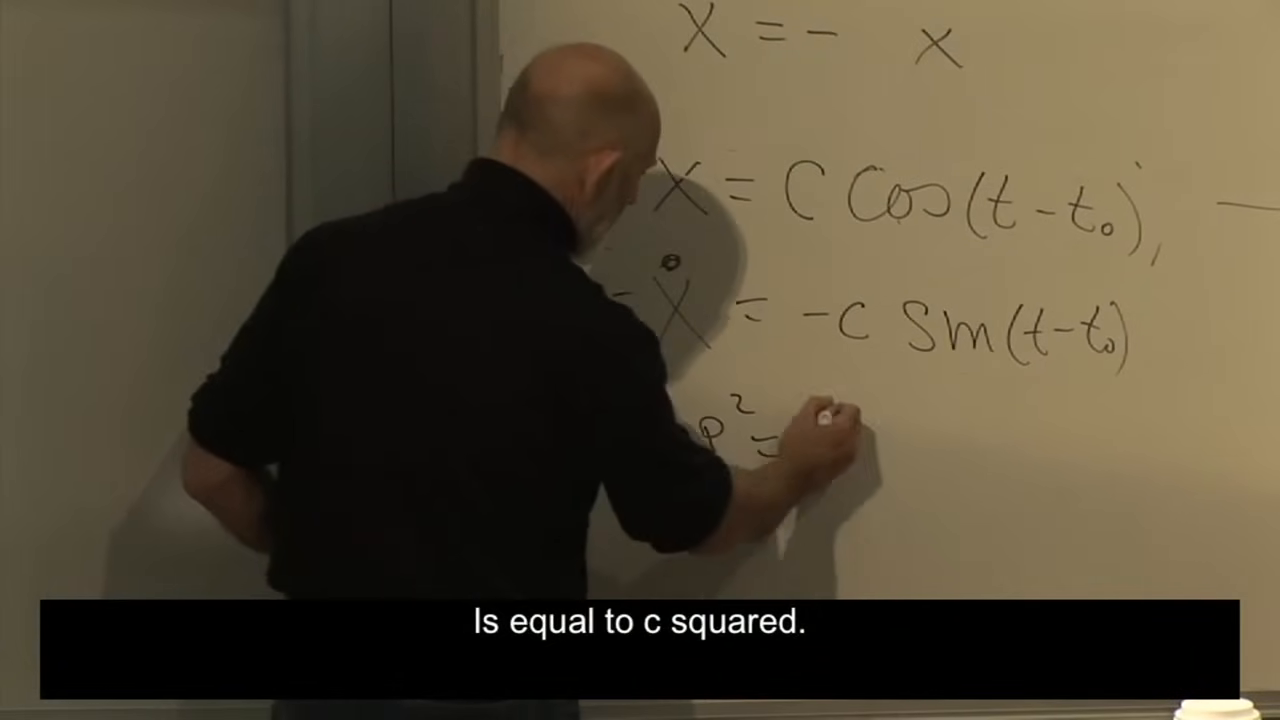
\includegraphics[width=0.84\textwidth]{lecture_02_figure_10.png}
  \caption{振動子の解と、\((x,p)\)位相平面におけるその円軌道。}
  \lectureframe{00:43:20}
\end{figure}

\begin{figure}[htbp]
  \centering
  \begin{tikzpicture}[scale=1.05,>=Latex]
    \draw[->] (-2.6,0) -- (2.75,0) node[right] {$x$};
    \draw[->] (0,-2.4) -- (0,2.55) node[above] {$p$};
    \draw[blue!65!black,thick] (0,0) circle (1.85);
    \draw[->,blue!65!black,thick]
      (1.60,0.93) arc[start angle=30,end angle=72,radius=1.85];
    \fill[red!65!black] (1.60,0.93) circle (2pt);
    \draw[dashed] (0,0) -- (1.60,0.93)
      node[midway,below right] {$C$};
    \node[align=left] at (-1.55,1.85)
      {$x=C\cos(t-t_0)$\\$p=-C\sin(t-t_0)$};
  \end{tikzpicture}
  \caption{位相空間の軌道は位置と運動量の両方を保持する。その半径は運動を特徴づけ、角度は時間とともに一様に進む。}
  \label{fig:oscillator-phase-space}
\end{figure}

水平軸への射影は\(x\)のよく知られた往復運動を与え、垂直軸への射影は\(p\)の振動を与える。アリストテレス的なばねとは異なり、異なる円が互いに崩れ合うことは決してない。位相空間の点が分かれば、その未来と過去の両方が決まる。

一般の\(m\)と\(k\)に対して、角振動数は

\begin{equation}
  \omega=\sqrt{\frac{k}{m}},
  \qquad
  x(t)=C\cos\bigl(\omega(t-t_0)\bigr),
  \label{eq:general-oscillator-frequency}
\end{equation}

であり、位相空間の軌道は規格化されていない\((x,p)\)平面では楕円になる。円の描像は、講義で用いた便利な\(m=k=1\)という規格化である。

\begin{classroomqa}
  \audiencequestion{振動子方程式の2階微分を1階微分に置き換えたら、予測可能性は失われるだろうか。\lecturetimestamp{00:45:23--00:46:04}}
  \lecturerresponse{いいえ。1階の方程式でも、適切な初期データから前方への運動を予測できる。より強い問題は、その流れが可逆であるのに十分なほど区別を保つかどうかである。関連する一般定理は、必要な道具が揃うまで保留する。}
\end{classroomqa}

\section{時間反転}

振動子の描像は可逆性を具体的にするが、方程式に対する直接的な検証もある。反転した時間座標を導入すると

\begin{equation}
  T=-t.
  \label{eq:reverse-time}
\end{equation}

このとき

\begin{equation}
  \frac{d}{dt}=-\frac{d}{dT},
  \qquad
  \frac{d^2}{dt^2}=\frac{d^2}{dT^2}.
  \label{eq:time-derivative-parity}
\end{equation}

1階微分は時間反転の下で符号を変えるが、2階微分は変えない。したがって、自律的なアリストテレス方程式

\begin{equation}
  m\dot x=F(x)
  \label{eq:aristotle-time-reversal}
\end{equation}

は、映画を逆再生してもその形を保たない。減衰するばねは、平衡から自発的に離れるばねになってしまう。対照的に、

\begin{equation}
  m\ddot x=F(x)
  \label{eq:newton-time-reversal}
\end{equation}

は変わらない。ニュートン的な映画を反転すると速度は反転するが加速度は変わらないので、逆再生の映画も別の許された解である。

\begin{figure}[htbp]
  \centering
  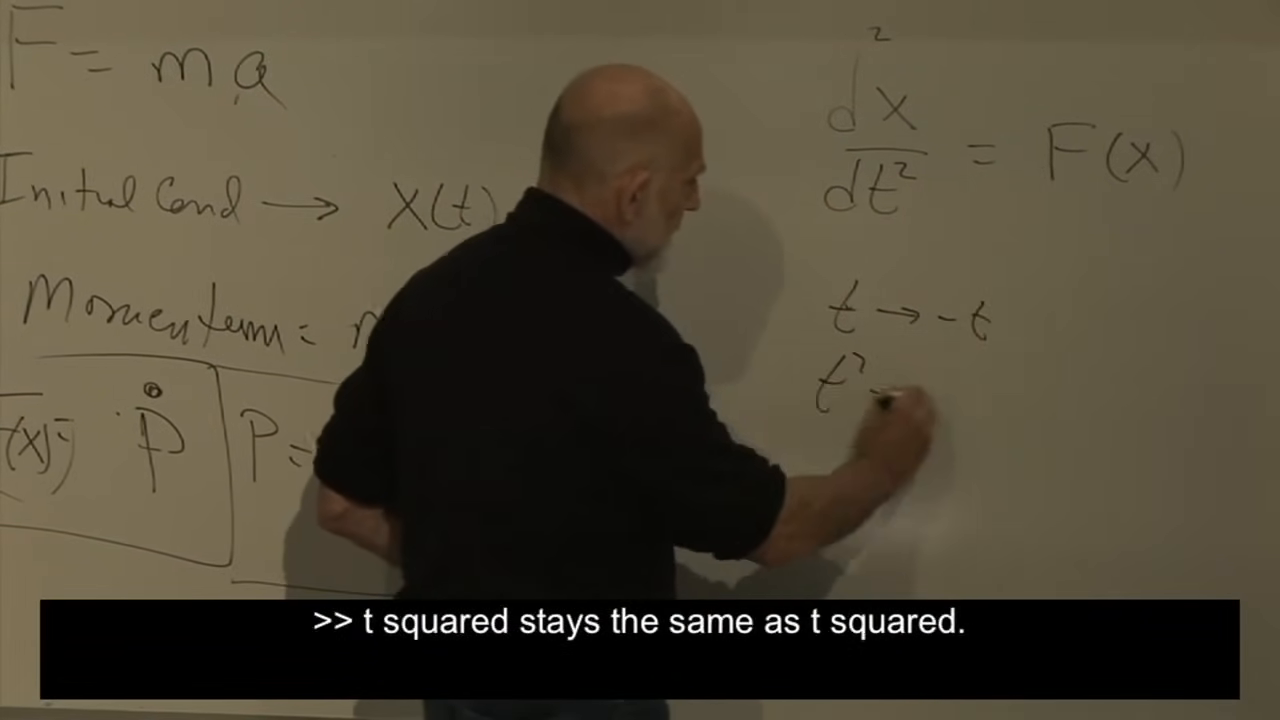
\includegraphics[width=0.84\textwidth]{lecture_02_figure_11.png}
  \caption{\(t\mapsto -t\)の下での板書の比較：1階微分は符号を反転するが、2階微分はそうしない。}
  \lectureframe{00:50:45}
\end{figure}

\begin{classroomqa}
  \audiencequestion{なぜ可逆性が一般に物理学についての前提として受け入れられるべきなのか。\lecturetimestamp{00:46:16--00:48:26}}
  \lecturerresponse{それは定義によって保証されるのではなく、検証されるものである。成功した法則を調べ、共通する実験的特徴を特定し、それらの特徴を原理へと高める。より深い論理的順序は逆方向に走る。量子場の理論の方がより基本的であり、ニュートン力学は低速運動や重い物体といった近似を通じて現れる。講義はより単純な法則から積み上げなければならないので、可逆性は今、その到達範囲が後に検証される原理として導入される。}
\end{classroomqa}

\begin{classroomqa}
  \audiencequestion{可逆性それ自体は、ニュートンが意識的に認識していた問題だったのか。\lecturetimestamp{00:48:28--00:49:02}}
  \lecturerresponse{歴史的な答えは不確かである。ニュートンが慣性を理解していたことは確かである。運動状態を変えるには力が必要であり、一様な運動を維持するには必要ない。彼がその洞察を可逆性の観点で明示的に定式化したかどうかは、別の歴史的問題である。}
\end{classroomqa}

\section{循環と保存量}

位相空間の円は次の考えを示唆する。軌道は1つの円上にとどまり、別の円へ跳ぶことは決してない。したがって、その円は運動に沿って一定に保たれる数でラベル付けできる。規格化された振動子では、その数は

\begin{equation}
  C^2=x^2+p^2.
  \label{eq:cycle-label}
\end{equation}

2分の1の因子を除けば、これは振動子のエネルギーである。より大きな円はより大きなエネルギーを持つ。出発位相を変えてもそれは変わらない。この主張は単に描像から読み取るのではなく導出するが、まず運動量を考える。

ニュートンの第1法則は、正味の力を受けない物体は一定の速度で運動すると述べている。それはすでに第2法則に含まれている：

\begin{equation}
  \mathbf F=0
  \quad\Longrightarrow\quad
  \dot{\mathbf p}=0
  \quad\Longrightarrow\quad
  \mathbf v=\text{constant}
  \label{eq:newton-first-from-second}
\end{equation}

質量が一定の場合について。ニュートンの第3法則は、粒子間の相互作用について真に新しい情報をもたらす。

\subsection{等しく、逆向きで、中心力である力}

粒子\(i\)が粒子\(j\)から受ける力を\(\mathbf F_{ij}\)と表す。第三法則の等しく逆向きの部分は

\begin{equation}
  \mathbf F_{ij}=-\mathbf F_{ji}.
  \label{eq:newton-third-pair}
\end{equation}

もし二つの力が同じ向きを向いていれば、孤立した対は自発的に加速し得る。それは内部の力だけから運動を生み出す、推進剤を使わない機械となるであろう。そのような振る舞いは観測されていない。

\begin{figure}[htbp]
  \centering
  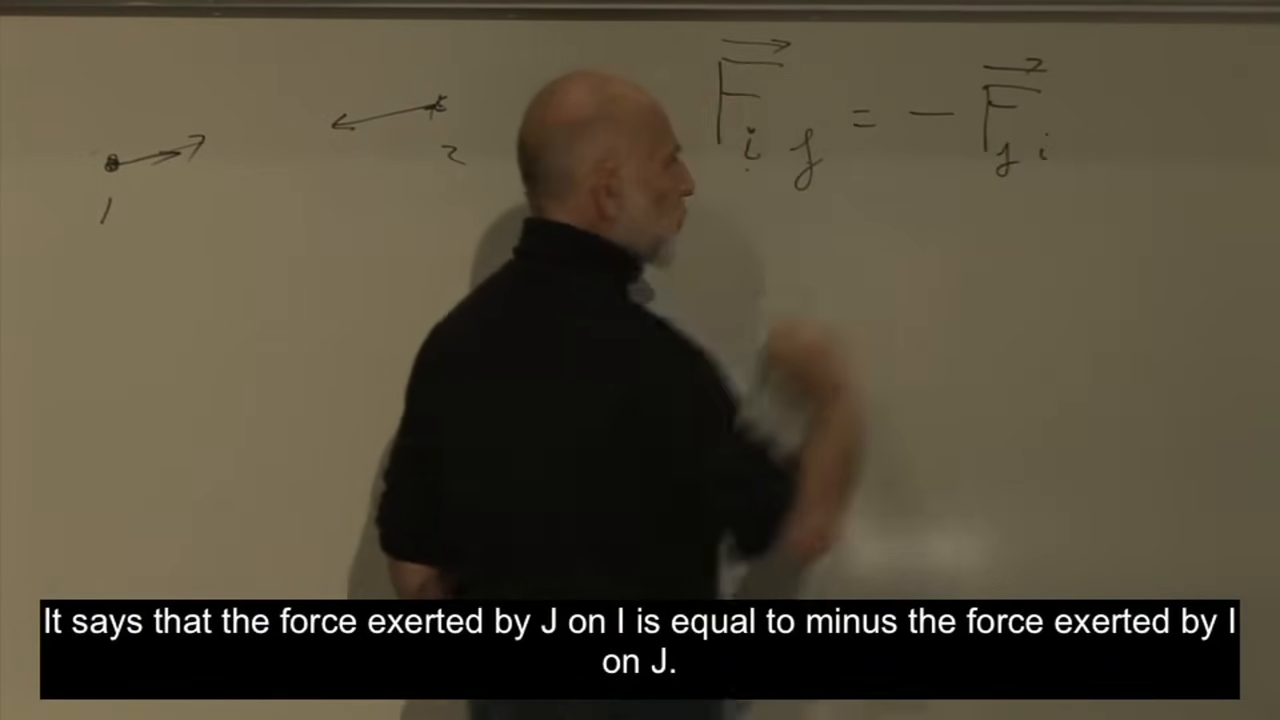
\includegraphics[width=0.84\textwidth]{lecture_02_figure_12.png}
  \caption{等しく逆向きの相互作用力の添字付き表現。}
  \lectureframe{00:59:25}
\end{figure}

ここで考える点粒子の力に対しては、その対は粒子中心を結ぶ線に沿っても働く。共線的でない等しく逆向きの力は純粋なトルクを形成し、孤立した剛体の対を回転させ始める可能性がある。中心力の条件はその可能性を防ぐ：

\begin{equation}
  \mathbf F_{ij}\parallel
  (\mathbf r_i-\mathbf r_j).
  \label{eq:central-force-condition}
\end{equation}

等しく逆向きの条件は線運動量の保存を与える。中心線の条件は角運動量の保存と結びついており、それは後に学ぶ。

\begin{figure}[htbp]
  \centering
  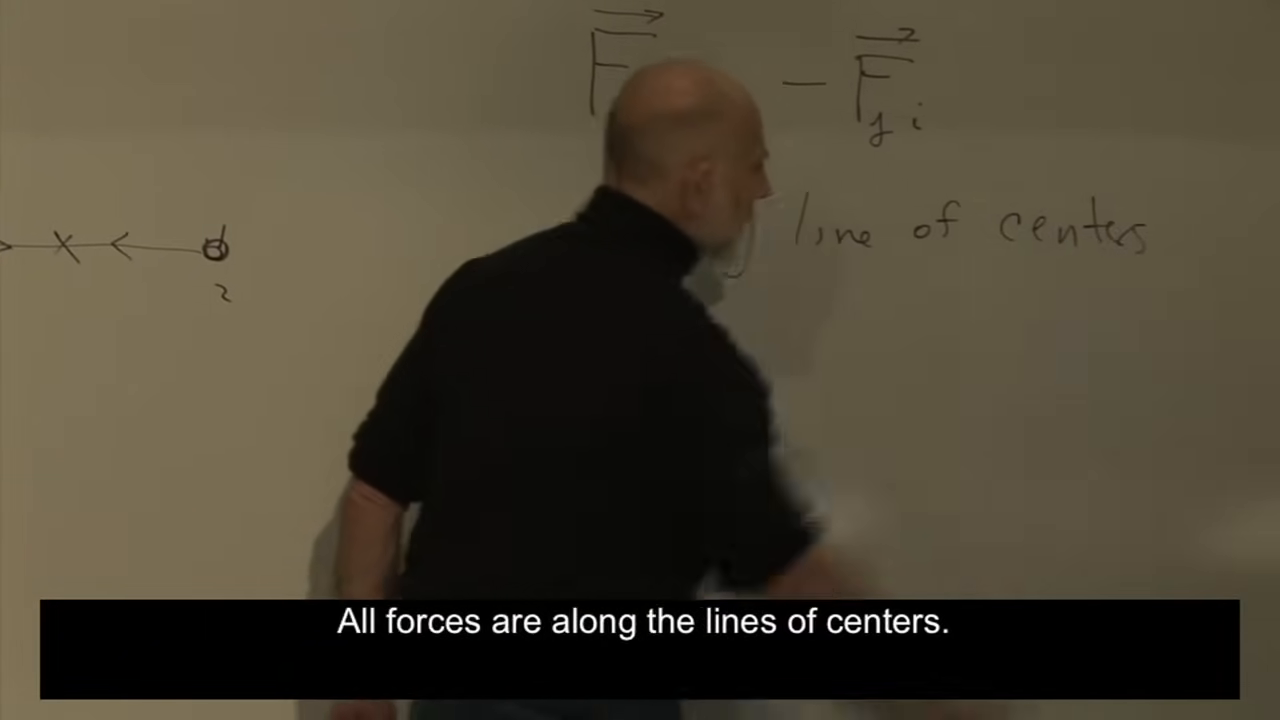
\includegraphics[width=0.84\textwidth]{lecture_02_figure_13.png}
  \caption{ニュートンの第三法則の中心力部分：相互作用力は粒子を結ぶ線に沿って働く。}
  \lectureframe{01:01:38}
\end{figure}

\subsection{全運動量}

\(N\)個の粒子からなる閉じた系を考える。外力はなく、力は粒子が互いに及ぼし合うものだけである。力の加法性とニュートンの第二法則により、各粒子について

\begin{equation}
  \dot{\mathbf p}_i
  =m_i\ddot{\mathbf r}_i
  =\sum_{\substack{j=1\\j\ne i}}^N \mathbf F_{ij}.
  \label{eq:many-particle-newton}
\end{equation}

この式を\(i\)について総和する：

\begin{align}
  \frac{d}{dt}\sum_{i=1}^N\mathbf p_i
  &=\sum_{i=1}^N
    \sum_{\substack{j=1\\j\ne i}}^N\mathbf F_{ij}
  \notag\\
  &=\sum_{i<j}\bigl(\mathbf F_{ij}+\mathbf F_{ji}\bigr)
  =0.
  \label{eq:momentum-pair-cancellation}
\end{align}

すべての相互作用は二度現れ、各方向に一度ずつ現れ、その対は相殺される。定義すると

\begin{equation}
  \mathbf P_{\mathrm{tot}}=\sum_{i=1}^N\mathbf p_i,
  \label{eq:total-momentum}
\end{equation}

最初の保存法則が得られる：

\begin{equation}
  \frac{d\mathbf P_{\mathrm{tot}}}{dt}=0.
  \label{eq:momentum-conservation}
\end{equation}

\begin{figure}[htbp]
  \centering
  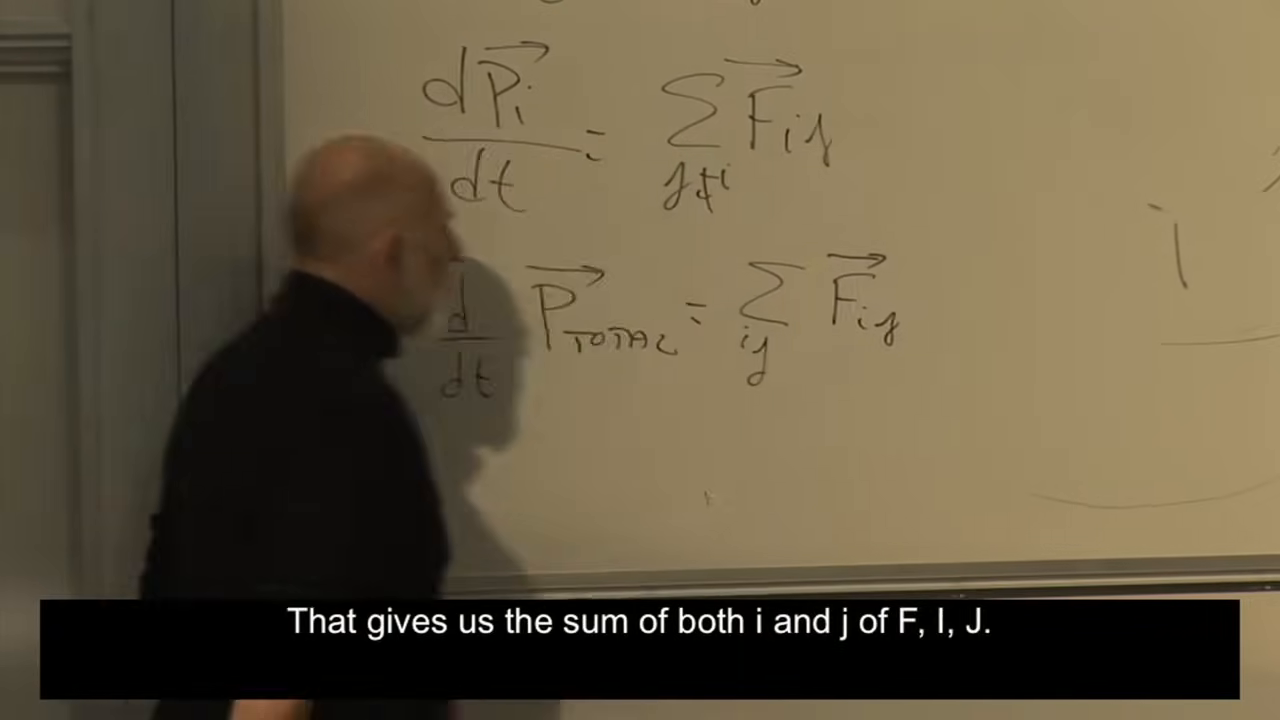
\includegraphics[width=0.84\textwidth]{lecture_02_figure_14.png}
  \caption{粒子の式を総和すると対の力が相殺され、全運動量の導関数がゼロに等しいままとなる。}
  \lectureframe{01:04:38}
\end{figure}

歴史的には、運動量保存をニュートンの第三法則の帰結として提示してきた。現代物理学では、運動量保存をより基本的な命題と見なすことが多い：孤立した二粒子系が全運動量を保存するならば、その内部運動量の変化は等しく逆向きでなければならない。しかし現在の展開には、ニュートン的な道筋が有用である。

\section{一次元におけるエネルギー}

その位置のみに依存する力の下で直線上を運動する一つの粒子を考える：

\begin{equation}
  F=F(x).
  \label{eq:position-force}
\end{equation}

このような力は時間に依存しないと呼ばれる。これは運動する粒子が経験する力の数値が一定であることを意味しない。その値は\(x(t)\)が変化するにつれて変化する。これは、粒子が同じ位置\(x\)にあるときはいつでも、時計の時刻に関係なく同じ力を受けることを意味する。

一次元では、十分に正則な力の関数は積分できる。したがってポテンシャルエネルギー\(V(x)\)を次で定義する：

\begin{equation}
  F(x)=-\frac{dV}{dx},
  \label{eq:potential-definition-1d}
\end{equation}

あるいは等価的に

\begin{equation}
  V(x)=-\int^x F(u)\,du+V_0.
  \label{eq:potential-integral}
\end{equation}

付加定数\(V_0\)は力に影響しない。\(V(x)\)を\(x\)軸の上にある景観の高さとして思い描く。粒子はより低い高さへ押され、傾きが急なほど力は大きい。滑らかな丘の頂上や底では傾きが消えるので、そこでは力も消える。

\begin{figure}[htbp]
  \centering
  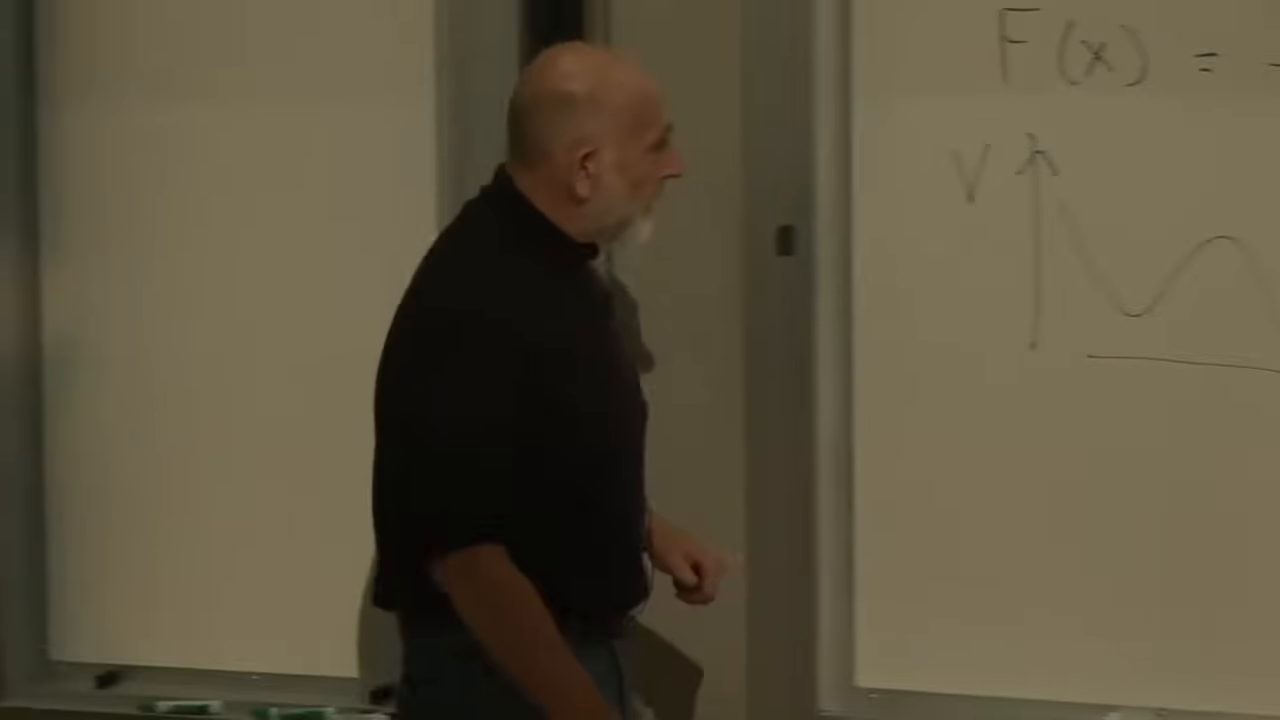
\includegraphics[width=0.84\textwidth]{lecture_02_figure_15.png}
  \caption{一次元の景観としてのポテンシャルエネルギー。力は下り坂を向き、その大きさは傾きによって定まる。}
  \lectureframe{01:12:57}
\end{figure}

運動エネルギー、ポテンシャルエネルギー、全エネルギーを次で定義する：

\begin{equation}
  T=\frac12m\dot x^2,
  \qquad
  E=T+V(x)
  =\frac12m\dot x^2+V(x).
  \label{eq:energy-1d}
\end{equation}

この段階では、エネルギーとはこの保存量の候補に与えられた名前にすぎない。その物理的解釈は景観によって示唆される：下り坂を転がると\(V\)が下がり、速度が増すので\(T\)が増す；上り坂を登ると逆になる。ニュートンの方程式はその交換が正確であることを証明する。

式~\eqref{eq:energy-1d}を微分する。\(m\)は定数であり、\(V\)は\(x(t)\)を通じてのみ時間に依存するので、

\begin{align}
  \frac{dE}{dt}
  &=m\dot x\ddot x+\frac{dV}{dx}\dot x
  \notag\\
  &=\dot x\left(m\ddot x+\frac{dV}{dx}\right).
  \label{eq:energy-derivative-1d}
\end{align}

ニュートンの法則と\(V\)の定義により

\begin{equation}
  m\ddot x=F=-\frac{dV}{dx}.
  \label{eq:newton-potential-1d}
\end{equation}

したがって式~\eqref{eq:energy-derivative-1d}の括弧は消える：

\begin{equation}
  \frac{dE}{dt}=0.
  \label{eq:energy-conservation-1d}
\end{equation}

\begin{figure}[htbp]
  \centering
  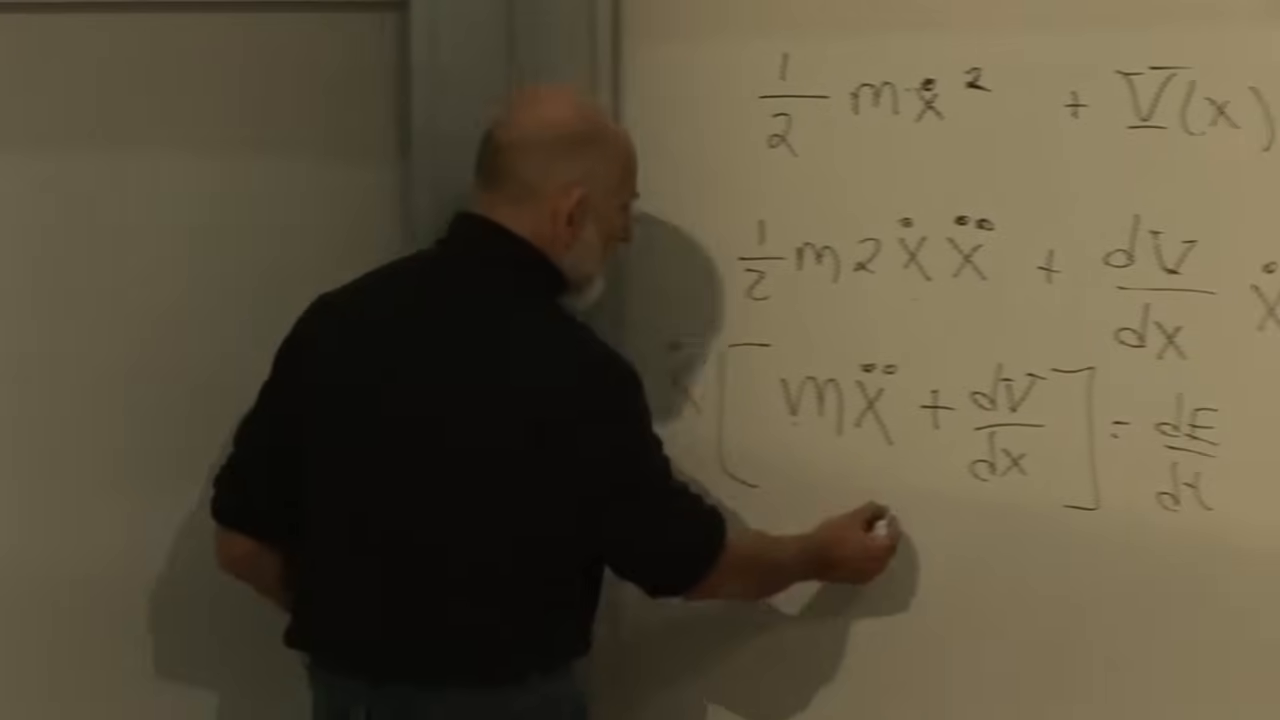
\includegraphics[width=0.84\textwidth]{lecture_02_figure_16.png}
  \caption{一次元のエネルギーの導関数は速度とニュートンの方程式の積に因数分解された。}
  \lectureframe{01:19:18}
\end{figure}

一次元では、正則な位置依存の力以外に追加の力学的前提は必要なかった。そのような力はすべて原始関数をもつからである。

\section{多次元と保存力}

座標\(x_i\)をもつ一つの粒子について、ニュートンの方程式は成分をもつ：

\begin{equation}
  F_i(\mathbf x)=m\ddot x_i.
  \label{eq:newton-components}
\end{equation}

力の成分\(F_i\)は\(x_i\)だけでなくすべての座標に依存し得る。次を満たす一つのスカラー関数\(V(\mathbf x)\)を見つけたい：

\begin{equation}
  F_i(\mathbf x)
  =-\frac{\partial V(\mathbf x)}{\partial x_i},
  \qquad
  \mathbf F=-\boldsymbol\nabla V.
  \label{eq:gradient-force}
\end{equation}

一次元の場合の構成とは異なり、これは自動的には成り立たない。三つの任意関数\(F_1,F_2,F_3\)は一般に、一つのスカラー関数の導関数よりも多くの独立な情報を含んでいる。等価に言えば、ポテンシャルが存在するのは、力の場が適切な混合偏導関数の等しさのような整合条件を満たす場合のみであり、単連結領域ではこれは\(\boldsymbol\nabla\times\mathbf F=0\)で表される。
したがって、式~\eqref{eq:gradient-force}を、考察対象の力のクラスに対する物理的要請として採用するのであり、数学的恒等式としてではない。

\begin{figure}[htbp]
  \centering
  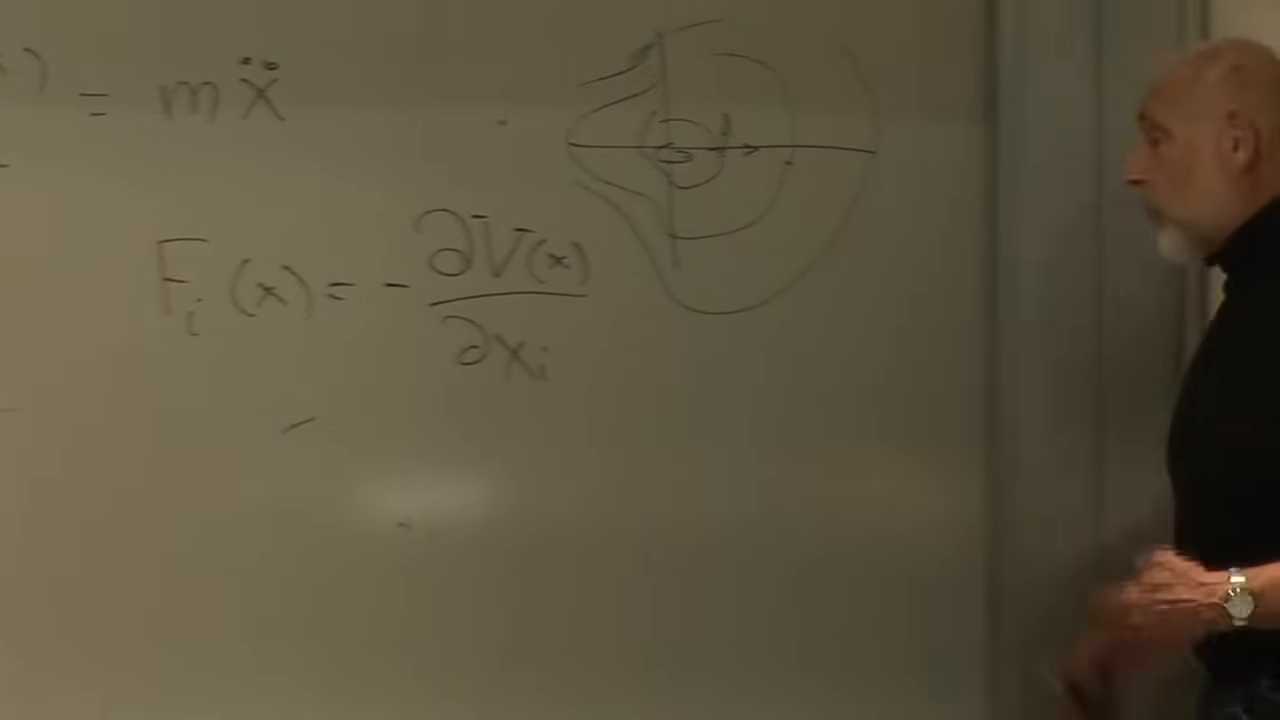
\includegraphics[width=0.84\textwidth]{lecture_02_figure_17.png}
  \caption{多次元の力の法則とポテンシャルの等高線スケッチ。力はレベル曲線を横切って\(V\)が減少する向きを指す。}
  \lectureframe{01:24:15}
\end{figure}

等高線図上では、\(V\)は各レベル曲線に沿って一定である。勾配はそれらの曲線に垂直で、最も急な増加の向きを指す。力\(-\boldsymbol\nabla V\)は最も急な減少の向きを指す。

\begin{figure}[htbp]
  \centering
  \begin{tikzpicture}[scale=1.0,>=Latex]
    \draw[->] (-3.0,0) -- (3.1,0) node[right] {$x_1$};
    \draw[->] (0,-2.4) -- (0,2.55) node[above] {$x_2$};
    \draw[orange!65!black,thick]
      plot[smooth cycle] coordinates
      {(-0.55,-0.35) (0.15,-0.55) (0.72,-0.10) (0.50,0.53) (-0.25,0.65)};
    \draw[orange!65!black,thick]
      plot[smooth cycle] coordinates
      {(-1.15,-0.75) (0.20,-1.10) (1.35,-0.25) (1.10,0.95) (-0.45,1.25)};
    \draw[orange!65!black,thick]
      plot[smooth cycle] coordinates
      {(-1.85,-1.20) (0.15,-1.70) (2.15,-0.40) (1.70,1.50) (-0.80,1.85)};
    \draw[->,blue!65!black,very thick] (1.62,0.73) -- (0.82,0.20)
      node[midway,above left] {$\mathbf F$};
    \draw[dashed,->,red!65!black,thick] (0.82,0.20) -- (1.62,0.73)
      node[midway,below right] {$\boldsymbol\nabla V$};
    \node[orange!65!black] at (-1.62,1.45) {$V=V_3$};
    \node[orange!65!black] at (-0.92,0.92) {$V=V_2$};
    \node[orange!65!black] at (-0.35,0.30) {$V=V_1$};
  \end{tikzpicture}
  \caption{スカラーポテンシャルのレベル曲線。勾配は等高線に法線であり、保存力は反対向きを指す。}
  \label{fig:potential-contours}
\end{figure}

式~\eqref{eq:gradient-force}が成り立つとき、次を定義する。

\begin{equation}
  E=\frac12m\sum_i\dot x_i^2+V(x_1,\ldots,x_n).
  \label{eq:energy-many-coordinates}
\end{equation}

運動項は質量の半分に速度ベクトルの長さの二乗を掛けたものである。微分し、多変数の連鎖律を適用すると次を得る。

\begin{align}
  \frac{dE}{dt}
  &=m\sum_i\dot x_i\ddot x_i
    +\sum_i\frac{\partial V}{\partial x_i}\dot x_i
  \notag\\
  &=\sum_i\dot x_i
    \left(m\ddot x_i+\frac{\partial V}{\partial x_i}\right)
  =0.
  \label{eq:energy-derivative-multidimensional}
\end{align}

証明は一次元の証明に添字を付けただけのものであるが、その前提はより強い。すなわち、力の成分はすべて一つのポテンシャルから生じなければならない。

\begin{figure}[htbp]
  \centering
  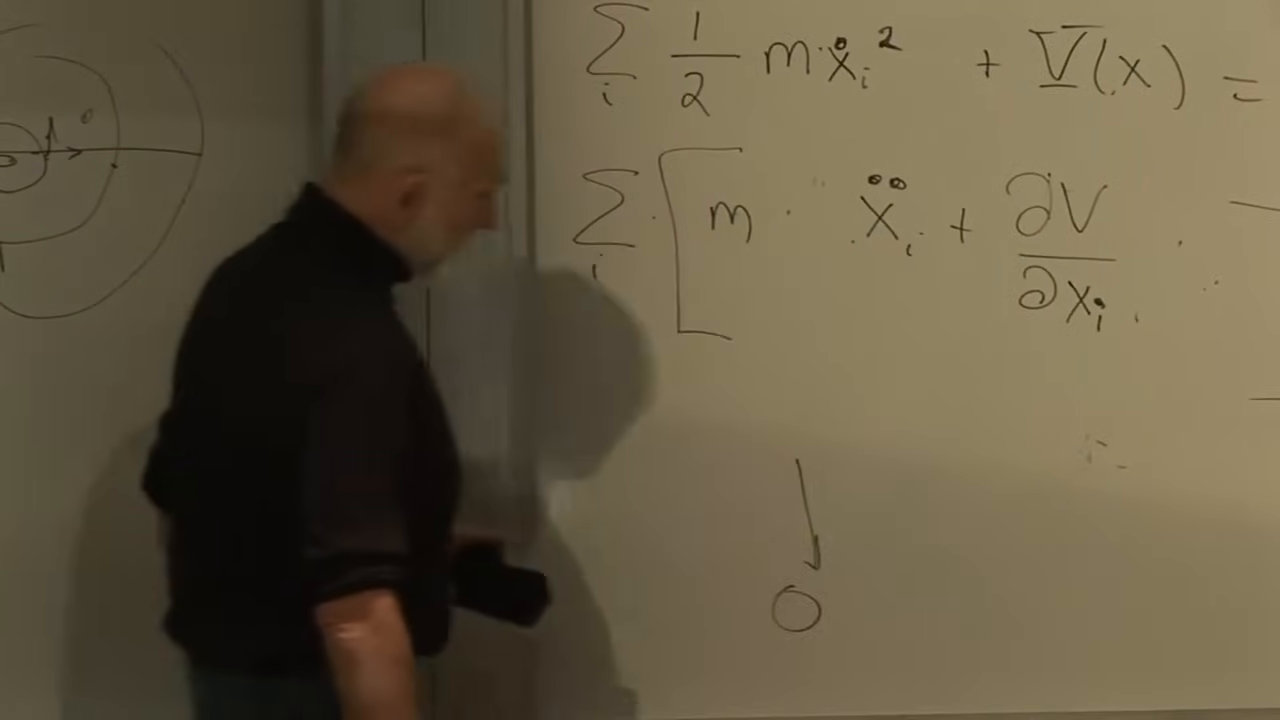
\includegraphics[width=0.84\textwidth]{lecture_02_figure_18.png}
  \caption{添字付きのエネルギー微分。各括弧はニュートン方程式の対応する成分によって消える。}
  \lectureframe{01:28:30}
\end{figure}

三次元の\(N\)個の粒子に対して、すべての座標を一つのリストにまとめる。

\begin{equation}
  \begin{aligned}
    q_a={}&(x_1,y_1,z_1,x_2,y_2,z_2,\ldots,\\[-0.2em]
           &\phantom{(}x_N,y_N,z_N),\\
    &a=1,\ldots,3N.
  \end{aligned}
  \label{eq:flattened-coordinates}
\end{equation}

\(3N\)個の座標成分があるが、粒子の質量は\(N\)個しかない。同じ質量が、ある与えられた粒子に属する三つの成分に現れる。もし

\begin{equation}
  F_a=-\frac{\partial V(q_1,\ldots,q_{3N})}{\partial q_a},
  \label{eq:many-particle-conservative-force}
\end{equation}

ならば

\begin{equation}
  E=\sum_{A=1}^{N}\frac12m_A\lvert\dot{\mathbf r}_A\rvert^2
    +V(\mathbf r_1,\ldots,\mathbf r_N)
  \label{eq:many-particle-energy}
\end{equation}

は同じ計算によって保存される。ポテンシャルから生じる力が\emph{保存力}と呼ばれるのは、まさにこの保存則を支えるからであり、この形容詞に政治的な意味はない。

\section{エネルギー等高線としての振動子}
\enlargethispage{3\baselineskip}

ばねの力\(F=-kx\)に対して、式~\eqref{eq:potential-definition-1d}は次を与える。

\begin{equation}
  V(x)=\frac12kx^2+V_0.
  \label{eq:spring-potential}
\end{equation}

\(V_0=0\)を選ぶと、振動子のエネルギーは次となる。

\begin{equation}
  E=\frac12m\dot x^2+\frac12kx^2
   =\frac{p^2}{2m}+\frac12kx^2.
  \label{eq:oscillator-energy}
\end{equation}

\(m=k=1\)に対して、

\begin{equation}
  2E=p^2+x^2=C^2.
  \label{eq:oscillator-energy-circle}
\end{equation}

したがって、以前に見出した位相空間の円は一定エネルギーの等高線である。より一般的な一次元ポテンシャルでは、等高線は円である必要はないが、運動は依然として曲線上にある。

\begin{equation}
  \frac{p^2}{2m}+V(x)=E
  \label{eq:general-energy-contour}
\end{equation}

\((x,p)\)平面において。これは第一回の講義の考えに戻る。すなわち、軌道が異なる周期や軌道にとどまるならば、ある数がそれらの軌道をラベル付けし、運動の間ずっと変わらずにいられる。

これで状態空間、ニュートン的な更新方程式、そして最初の二つの保存則が揃った。力学の次の定式化は最小作用の原理から始まり、ラグランジアン、ハミルトニアン、角運動量、そしてこれらの例の背後にあるより一般的な構造へと導くであろう。

\begin{classroomqa}
  \audiencequestion{配布された資料と板書の内容はどの程度一致しているのか、そして図はどこにあるのか。\lecturetimestamp{01:37:56--01:38:54}}
  \lecturerresponse{資料は講義に忠実に従うはずである。板書にある内容が欠けていれば、間違ったファイルが送られた可能性がある。図はまだ準備されていなかった。彼が冗談めかして言うには、継続教育課程が次の小切手を支払ったときに現れるだろうとのことだった。}
\end{classroomqa}